\documentclass[12pt,a4paper]{report}
\usepackage[utf8]{inputenc}
\usepackage{graphicx}
\usepackage{amsmath}
\usepackage{hyperref}
\usepackage{listings}
\usepackage{xcolor}

% Configuración para Python
\lstset{
    language=Python,               % Lenguaje del código
    basicstyle=\ttfamily\footnotesize,  % Tipo de letra
    keywordstyle=\color{blue},     % Color de las palabras clave
    commentstyle=\color{green},    % Color de los comentarios
    stringstyle=\color{red},       % Color de los strings
    numbers=left,                  % Mostrar números de línea
    numberstyle=\tiny\color{gray}, % Estilo de los números de línea
    stepnumber=1,                  % Número de líneas entre números de línea
    frame=single,                  % Marco alrededor del código
    breaklines=true,               % Partir líneas largas
    showstringspaces=false         % No mostrar espacios en los strings
}

\title{Informe Problema 2}
\author{
    Marco Antonio Ochil Trujillo \\
    \and
    Kevin Majim Ortega Alvarez \\
    \and
    Yoan Rene Ramos Corrales \\
}
\date{September 23, 2024}

\begin{document}

\maketitle

\tableofcontents

\chapter{Problema}

\textbf{Dos contadores}

Tienes 2 contadores $a$ y $b$, ambos inicializados en 0. También tienes un puntaje inicializado en 0.

Al inicio de cada minuto, desde el minuto 1 hasta el minuto $N$, debes incrementar ya sea $a$ o $b$ en 1.

Adicionalmente, hay $M$ eventos. El evento $i$ ocurre en el minuto $T_i + 0.5$ y tiene tipo $C_i$ $(C_i \in \{1, 2\})$.

En cada evento, los contadores o el puntaje se actualizan de la siguiente manera:

\begin{lstlisting}
if (type == 1):
    if (a > b):
        score = score + 1;
    else:
        a = 0;
        b = 0;
else:
    if (a < b):
        score = score + 1;
    else:
        a = 0;
        b = 0;
\end{lstlisting}

Tu tarea es maximizar el puntaje después de que hayan pasado $N$ minutos.

\chapter{Soluciones}

\section{Algoritmo de Fuerza Bruta}

En cada iteración se calcula que pasaría si aumentáramos $a$ o $b$ con una función recursiva que tiene como caso de parada el momento en que se llega al final del tiempo posible, comparando luego el $score$ obtenido con el máximo encontrado hasta el momento.

Para $time = 1$ comprobamos el caso de aumentar $a$ y el caso de aumentar $b$ que son todos los casos posibles en una iteración y por cada uno de ellos revisamos todos los posibles en las siguientes iteraciones, que se hace analizando estos mismos dos casos en cada iteración. Luego no quedan casos sin revisar en el algoritmo recursivo y como este actualiza el $score$ máximo al final de cada camino, se asegura que el camino al finalizar el algoritmo es de $score$ máximo.

En cada iteración se analizan dos casos y basándose en estos se realiza la iteración siguiente en la que también se analizan dos casos, esto se hace $N$ veces, luego la complejidad temporal de este algoritmo es $O(2^N)$$.

\section{Algoritmo Greedy}

Este algoritmo fue nuestra primera idea de la solución, desafortunadamente no era la correcta. No utilizaba las variables $a$, $b$ sino su factor de balance: $Fb = a – b$. Se definió un rango de factores de balance posible $|Fb| \leq 2$ y se creó un autómata de 5 estados utilizando el $Fb$, el tipo de evento del problema y las distancias entre dos eventos consecutivos. Para las distancias entre los eventos se tomó la siguiente función para generar una cadena:

\[
f(x) =
\begin{cases} 
x & \text{si } x \leq 2, \\
i & \text{si } x > 2 \land x \% 2 == 1, \\
p & \text{si } x > 2 \land x \% 2 == 0.
\end{cases}
\]

\smallskip

Con esto se generó un autómata que va a ser dividido con respecto al tipo de evento para simplificar su comprensión. El $Fb$ define el estado en que va a estar el problema teniendo como inicio a $Q0$ ya que es el valor del $Fb$ inicial:

\begin{figure}[h]  % Usamos el entorno figure
    \centering
    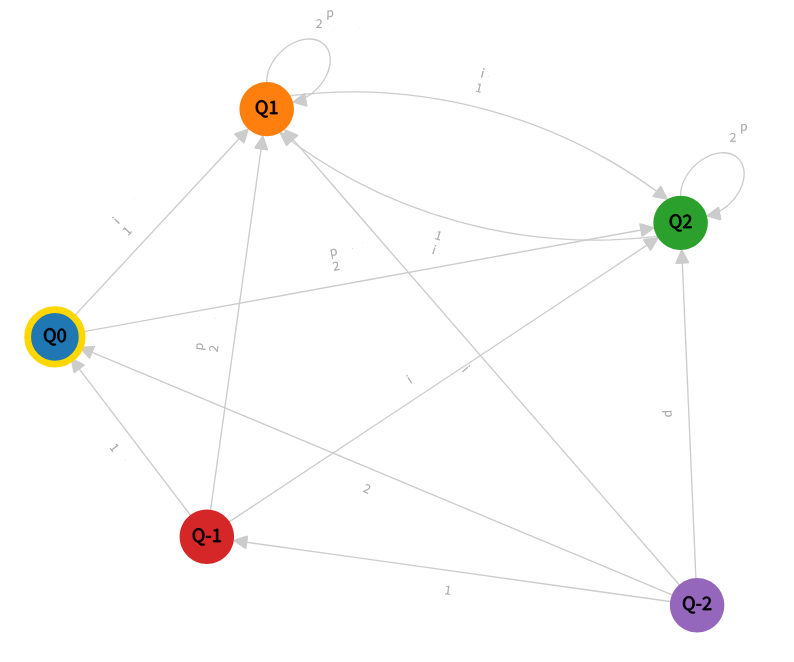
\includegraphics[width=\textwidth]{type 1.png}
    \caption{Evento de tipo 1.}
    \label{fig:type1}  % Etiqueta para referenciar la imagen
\end{figure}

\begin{figure}[h]  % Usamos el entorno figure
    \centering
    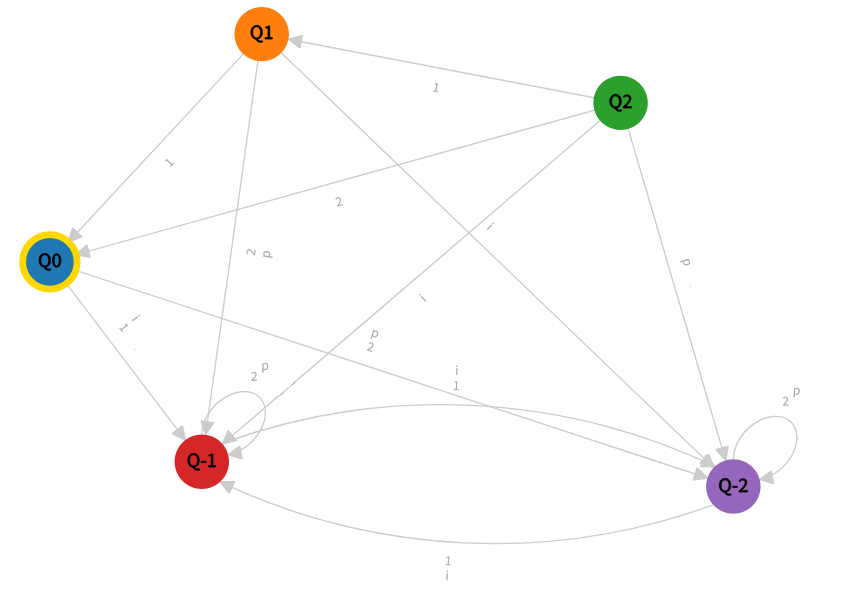
\includegraphics[width=\textwidth]{type 2.png}
    \caption{Evento de tipo 2.}
    \label{fig:type1}  % Etiqueta para referenciar la imagen
\end{figure}

En este algoritmo se tenía que precomputar las distancias entre cada par de eventos consecutivos lo que sería $O(M)$ y luego iterar entre los eventos, no entre minutos, utilizando los valores precomputados que comprimían la información sobre estos minutos, por lo que se realizaban $M$ iteraciones. Con esto podemos llegar a que el algoritmo se realizaba en $O(M)$.

Para este algoritmo se puede encontrar el siguiente contraejemplo:

\smallskip

\{1.5: 1,   2.5: 2,   4.5: 2,   6.5: 1,   7.5: 1,   9.5: 1,   10.5: 1,   11.5: 2\}

Donde las llaves son los $T_i$ de cada evento y los valores el tipo de evento, en este caso el Algoritmo Fuerza Bruta nos mostró que la mejor opción es perder el primer evento y conseguir del segundo al séptimo evento, con un $score$ de 6. Para nuestro Algoritmo Greedy la idea de dejar pasar el primer evento era impensable y decidimos cambiar nuestra perspectiva del problema por este caso.

\section{Algoritmo de Programación Dinámica}

Tenemos una matriz $dp$ de tamaño $N x (2*N) + 1$, donde cada fila $i$ representa al minuto $i$, mientras que cada columna $j$ representa al $Fb = j$, inicializada en 0; también tendremos un conjunto $x$ de $Fb$ posibles a los que podremos llegar en la iteración siguiente del algoritmo, o sea en la iteración $i$ se determina el conjunto de la iteración $i+1$.

El algoritmo inicia con esta matriz y con $x$ que solo contiene a 0 porque es el valor en que se inicia el problema, por cada valor $y$ en $x$ añadiremos a los valores $y+1$ y $y-1$ para la siguiente iteración y cambiaremos el valor de estos en $dp$ de la siguiente manera:

\smallskip

$dp[i+1][y-1] = max(dp[i+1][y-1], dp[i][y])$

$dp[i+1][y+1] = max(dp[i+1][y+1], dp[i][y])$

\smallskip

(esto en caso de no existir evento entre los minutos $i$ e $i+1$)

Se utiliza el máximo porque el valor de $dp[i+1][z]$ en principio puede ser modificado por los valores $z+1$ y $z-1$ de la iteración anterior, nos interesa solo quedarnos con el mayor.

Para el caso en que hay evento se evalua si los valores $y+1$ y $y-1$ cumplen el evento, en caso de que cumplan el evento se añaden al conjunto de iteración siguiente y se actualiza de la manera ya vista aumentando el $score$:

\smallskip

$dp[i+1][y-1] = max(dp[i+1][y-1], dp[i][y] + 1)$

$dp[i+1][y+1] = max(dp[i+1][y+1], dp[i][y] + 1)$

\smallskip

En caso contrario se añade al conjunto el valor 0 que es donde iniciaría este camino al no pasar el evento y no se actualizaría el valor correspondiente en $dp$, sino:

\smallskip

$dp[i+1][0] = max(dp[i+1][0], dp[i][y])$

\smallskip

Al finalizar las $N$ iteraciones nos quedamos con el valor máximo de la última fila de la matriz que será la máxima cantidad de eventos posibles a ganar.

\subsection{Demostración}

Queremos demostrar que conociendo el conjunto de los $Fb$ de la iteración $i$, sus valores de $score$ y la existencia o ausencia de evento en el minuto $i + 0.5$, podemos determinar el conjunto de $Fb$ posibles en la iteración $i+1$ y sus valores de $score$ máximo:

\bigskip

Caso base $i = 0$, $x = \{0\}$, $dp[0] = [0, 0, …, 0]$

\medskip

• Evento en 0.5 = False:

Para el minuto 1: $x = \{-1, 1\}$ pues no existe evento que pueda volver a 0 el valor del $Fb$

\smallskip

$dp[1][-1] = 0$ y $dp[1][1] = 0$

\medskip

• Evento en 0.5 = 1:

Para el minuto 1: $x = \{0, 1\}$ porque al aumentar el valor de $b$ y disminuir el $Fb$ no se cumplió con el primer evento

\smallskip

$dp[1][0] = 0$ y $dp[1][1] = 1$

\medskip

• Evento en 0.5 = 2:

Para el minuto 1: $x = \{-1, 0\}$ porque al aumentar el valor de $a$ y aumentar el $Fb$ no se cumplió con el primer evento

\smallskip

$dp[1][-1] = 1$ y $dp[1][0] = 0$

\bigskip

Caso inductivo $i$, $x = \{j, k, …, z\}$, $dp[i] = [p, q, …, r]$

\medskip

• Evento en $i.5$ = False:

Para el minuto $i+1$: $x = \{j-1, j+1, k-1, k+1, …, z-1, z+1\}$ pues no existe evento que pueda volver a 0 el valor del $Fb$, recordando siempre que $x$ es un conjunto y por tanto no existen valores repetidos.

con $dp[i+1][u] = max(dp[i+1][u], dp[i+1][u-1], dp[i+1][u+1])$ \forall $u$ \in $x_{i+1}$, sabiendo que ambos casos $u-1$ y $u+1$ no tienen porque existir en $x_i$, solo al menos uno de ellos es necesario para esto.

\medskip

• Evento en $i.5$ = 1:

Para el minuto $i+1$: $x_{i+1} = \{t | (t + 1 \lor t – 1 \in x_i \land t > 0) \lor (t = 0 \land \exists v < 1 | v \in x_i)\}$, se calcula el $score$ máximo para cada valor de $x_{i+1}$ de la manera explicada en el algoritmo.

\medskip

• Evento en $i.5$ = 2:

Para el minuto $i+1$: $x_{i+1} = \{t | (t + 1 \lor t – 1 \in x_i \land t < 0) \lor (t = 0 \land \exists v > 1 | v \in x_i)\}$, se calcula el $score$ máximo para cada valor de $x_{i+1}$ de la manera explicada en el algoritmo.

\bigskip

Con esto garantizamos que en cada iteración se están analizando todos los factores de balance posibles y actualizando correctamente sus valores de $score$. Este algoritmo realiza una iteración por cada minuto, serian $N$ iteraciones, dentro de cada una de estas inserta a lo sumo $2*N$ elementos en un conjunto, lo que sería $O(N*\log{N})$ además de analizar 2 casos por cada $Fb$, lo que sería a lo sumo $4*N + 2$ dada la cantidad máxima de $Fb$ posibles, luego su complejidad es $O(N*(N*\log{N} + 4*N))$ que es $O(N^{2}*\log{N})$.

Para esta demostración utilizamos por comodidad la matriz $dp$ de tamaño $Nx2*N +1$, pero basándonos en el algoritmo greedy cambiamos esta matriz a $N x 5$, considerando un $Fb$ restringido como se planteaba en este algoritmo, ya que cualquier factor de balance que se aleje de 0 es evidentemente contraproducente y todos los casos tratados con $|Fb| > 2$ son reducibles a $|Fb| \leq 2$. Con esto la complejidad temporal dentro de cada iteración se convierte en $O(5*\log{5} + 20)$ que es $O(c)$, luego quedaría en $O(N)$. 


\end{document}
